\documentclass{article}

% Required packages
\usepackage{amssymb}
\usepackage{amsmath}
\usepackage{graphicx}
\usepackage{geometry}
\usepackage{tikz}
\usepackage{array}
\usepackage{booktabs}
\usepackage{enumitem}
\usepackage{listings}
\usepackage{xcolor}
\usepackage{fancyhdr}
\usepackage{float}
\usepackage{subcaption}
\usepackage{comment}

% Set page geometry
\geometry{a4paper, margin=1in}

% Configure listings for Python
\lstset{
  language=Python,
  basicstyle=\ttfamily\footnotesize,
  numbers=left,
  numberstyle=\tiny\color{gray},
  frame=single,
  breaklines=true,
  breakatwhitespace=true,
  captionpos=b,
  tabsize=4,
  showspaces=false,
  showstringspaces=false,
  showtabs=false,
  commentstyle=\color{gray}\textit,
  keywordstyle=\color{blue}\bfseries,
  stringstyle=\color{red}
}

\begin{document}

\pagestyle{fancy}
\chead{DSC 257: Unsupervised Learning (Fall 2025)}
\lhead{Homework 2}
\rhead{Randall Rogers}

%------------------
% Solution for 1(a) 
%------------------
\subsection*{Solution 1}
\noindent\rule{\textwidth}{0.4pt}\\

\subsubsection*{Solution 1 (a)}
\subsubsection*{Define $\ell_1$}
\parbox{\textwidth}{
The $\ell_1$ or $||x||_1$ is defined as:
$$\ell_{1} = ||x||_1 = \sum_{i=1}^{d} |x_{i}| $$
}
\subsubsection*{Compute $\ell_1$}
\parbox{\textwidth}{
Let $x=\begin{bmatrix} 1 \\ -2 \\ 3 \end{bmatrix}$ \\

\begin{align*}
  ||x||_1 &= \sum_{i=1}^{3} |x_{i}| \\
  &= |x_{1}| + |x_{2}| + |x_{3}| \\
  &= |1| + |-2| + |3| \\
  &= 1 + 2 + 3 \\
  &= 6
\end{align*}
}


\subsubsection*{\normalfont}{$\therefore$ $||x||_{1} = 6$}

\noindent\rule{\textwidth}{0.4pt}\\

\newpage

%------------------
% Solution for 1(b) 
%------------------
\subsection*{Solution 1}
\noindent\rule{\textwidth}{0.4pt}\\

\subsubsection*{Solution 1 (b)}
\subsubsection*{Define $\ell_2$}
\parbox{\textwidth}{
The $\ell_2$ or $||x||_2$ is defined as:
$$\ell_{2} = ||x||_2 = \sqrt{\sum_{i=1}^{d} x_{i}^2} $$
}
\subsubsection*{Compute $\ell_2$}
\parbox{\textwidth}{
Let $x=\begin{bmatrix} 1 \\ -2 \\ 3 \end{bmatrix}$ \\

\begin{align*}
  ||x||_2 &= \sqrt{\sum_{i=1}^{3} x_{i}^{2}} \\
  &= \sqrt{x_{1}^2 + x_{2}^{2} + x_{3}^{2}} \\
  &= \sqrt{1^{2} + (-2)^{2} + 3^{2}} \\
  &= \sqrt{1 + 4 + 9} \\
  &= \sqrt{14}
\end{align*}
}


\subsubsection*{\normalfont}{$\therefore$ $||x||_{2} = \sqrt{14}$}

\noindent\rule{\textwidth}{0.4pt}\\

\newpage

%------------------
% Solution for 1(c) 
%------------------
\subsection*{Solution 1}
\noindent\rule{\textwidth}{0.4pt}\\

\subsubsection*{Solution 1 (c)}
\subsubsection*{Define $\ell_{\infty}$}
\parbox{\textwidth}{
The $\ell_{\infty}$ or $||x||_{\infty}$ is defined as:
$$\ell_{\infty} = ||x||_{\infty} = \text{max}_{i}\left|x_{i}\right| $$
}
\subsubsection*{Compute $\ell_{\infty}$}
\parbox{\textwidth}{
Let $x=\begin{bmatrix} 1 \\ -2 \\ 3 \end{bmatrix}$ \\

\begin{align*}
  ||x||_{\infty} &= \text{max}(\{|x_{1}|,|x_{2}|,|x_{3}|\}) \\
  &= \text{max}(\{|1|,|-2|,|3|\}) \\
  &= \text{max}(\{1,2,3\}) \\
  &= 3 \\
\end{align*}
}

\subsubsection*{\normalfont}{$\therefore$ $||x||_{\infty} = 3$}

\noindent\rule{\textwidth}{0.4pt}\\

\newpage


%------------------
% Solution for 2(a)
%------------------
\subsection*{Solution 2}
\noindent\rule{\textwidth}{0.4pt}\\
\subsubsection*{Solution 2 (a)}

\subsubsection*{Define $\ell_{2}$ distance}
\parbox{\textwidth}{The $\ell_2$ distance is defined as:
$$d(x, x^{\prime})_{\ell_2} = \sqrt{\sum_{i=1}^{n} (x_i-x_{i}^{\prime})^2}$$
}
\subsubsection*{Compute $\ell_{2}$ distance}
\parbox{\textwidth}{
Let $x = \begin{bmatrix} -1 \\ 1 \\ -1 \\ 1 \end{bmatrix}$ and $x^{\prime}=\begin{bmatrix} 1 \\ 1 \\ 1 \\ 1 \end{bmatrix}$
\begin{align*}
    d(x, x^{\prime})_{\ell_2} &= \sqrt{(x_{1}-x_{1}^{\prime})^2 + (x_{2}-x_{2}^{\prime})^2 + (x_{3}-x_{3}^{\prime})^2 + (x_{4}-x_{4}^{\prime})^2} \\
    &= \sqrt{((-1)-1)^2 + (1-1)^2 + ((-1)- 1)^2 + (1-1)^2} \\
    &= \sqrt{(2)^2 + (0)^2 + (2)^2 + (0)^2} \\
            &= \sqrt{4 + 0 + 4 + 0} \\
            &= \sqrt{8} 
\end{align*}
}
\subsubsection*{\normalfont}{$\therefore d(x, x^{\prime})_{\ell_2} = \sqrt{8}$}

\noindent\rule{\textwidth}{0.4pt}\\
\newpage

\subsection*{Solution 2}
\noindent\rule{\textwidth}{0.4pt}\\
\subsubsection*{Solution 2 (b)}

\subsubsection*{Define $\ell_{1}$ distance}
\parbox{\textwidth}{The $\ell_1$ distance is defined as:
$$d(x, x^{\prime})_{\ell_1} = \sum_{i=1}^{n} |x_i - x_{i}^{\prime}|$$
}
\subsubsection*{Compute $\ell_{1}$ distance}
\parbox{\textwidth}{
Let $x = \begin{bmatrix} -1 \\ 1 \\ -1 \\ 1 \end{bmatrix}$ and $x^{\prime}=\begin{bmatrix} 1 \\ 1 \\ 1 \\ 1 \end{bmatrix}$
\begin{align*}
    d(x, x^{\prime})_{\ell_1} &= |x_{1}-x_{1}^{\prime}| + |x_{2}-x_{2}^{\prime}| + |x_{3}-x_{3}^{\prime}| + |x_{4}-x_{4}^{\prime}| \\
    &= |-1 - 1| + |1 - 1| + |-1 - 1| + |1 - 1| \\
    &= |-2| + |0| + |-2| + |0| \\
    &= 2 + 0 + 2 + 0 \\
    &= 4
\end{align*}
}
\subsubsection*{\normalfont}{$\therefore d(x, x^{\prime})_{\ell_1} = 4$}

\noindent\rule{\textwidth}{0.4pt}\\

\newpage

\subsection*{Solution 2}
\noindent\rule{\textwidth}{0.4pt}\\
\subsubsection*{Solution 2 (c)}

\subsubsection*{Define $\ell_{\infty}$ distance}
\parbox{\textwidth}{The $\ell_\infty$ distance is defined as:
$$d(x, x^{\prime})_{\ell_\infty} = \max_{i} |x_i - x_{i}^{\prime}|$$
}
\subsubsection*{Compute $\ell_{\infty}$ distance}
\parbox{\textwidth}{
Let $x = \begin{bmatrix} -1 \\ 1 \\ -1 \\ 1 \end{bmatrix}$ and $x^{\prime}=\begin{bmatrix} 1 \\ 1 \\ 1 \\ 1 \end{bmatrix}$
\begin{align*}
    d(x, x^{\prime})_{\ell_\infty} &= \max\{|x_1 - x_1^{\prime}|, |x_2 - x_2^{\prime}|, |x_3 - x_3^{\prime}|, |x_4 - x_4^{\prime}|\} \\
    &= \max\{|-1 - 1|, |1 - 1|, |-1 - 1|, |1 - 1|\} \\
    &= \max\{|-2|, |0|, |-2|, |0|\} \\
    &= \max\{2, 0, 2, 0\} \\
    &= 2
\end{align*}
}
\subsubsection*{\normalfont}{$\therefore d(x, x^{\prime})_{\ell_\infty} = 2$}

\noindent\rule{\textwidth}{0.4pt}\\

\newpage

%------------------
% Solution for 3(a)
%------------------
\section*{Solution 3}
\noindent\rule{\textwidth}{0.4pt}\\
\subsection*{Solution 3 (a)}
\subsubsection*{(i) max($\ell_1$) given $\|x\|_{\infty}=1$}

%\subsubsection*{Find implications given $\|x\|_{\infty}=1$}
\begin{enumerate}
  \item Find implications given $\|x\|_{\infty}=1$

\begin{flushleft}
Given the constraint $\|x\|_{\infty} = \max_{i} |x_i| = 1$. It follows that $|x_i| \le 1$ : $\forall i \in \{1,2,...,d\}$ where $d$ is the dimension of vector $x$.
The $\ell_1$-norm, is the sum of the absolute values of the components($x_i$) in the vector $x$ or :
\end{flushleft}

$$\ell_1 = \sum_{i=1}^d |x_i| = |x_1| + |x_2| + \ldots + |x_d|$$ 
\begin{flushleft}
Each term $|x_i|$ in the sum must be maximized in order to maximaize $\ell_1$-norm. The given constraint($\|x\|_{\infty}=1$) allows each $|x_i|$ to be at most 1. Hence, the maximum is achieved when $|x_i|=1$ or $x_i=\pm1$.
\end{flushleft}
  \item Find value of $\ell_1$-norm
\end{enumerate}
\begin{align*}
    \|x\|_1 &= \sum_{i=1}^d |x_i| \\
    &\le \sum_{i=1}^d 1 \quad (\text{since } |x_i| \le \|x\|_{\infty} = 1) \\
    &\le d
\end{align*}

\subsubsection*{\normalfont}{$\therefore$ The vector $x = \begin{bmatrix} \pm 1 \\ \pm 1 \\ \vdots \\ \pm 1 \end{bmatrix}$ maximizes the norm, with a value of $\|x\|_1 = d$.}

\subsubsection*{(ii): Maximize $\|x\|_2$ given $\|x\|_{\infty}=1$}
\begin{enumerate}
  \item \parbox{\textwidth}{Apply part (i) results and solve for $\ell_2$-norm}
\begin{flushleft}
  Given the same constraint $\|x\|_{\infty} = 1$. From the results in part $(i)$:
\end{flushleft}
\end{enumerate}

\begin{align*}
    \|x\|_2 &= \sqrt{\sum_{i=1}^d x_i^2} \\
    &= \sqrt{\sum_{i=1}^d |x_i|} \quad (\text{since all} x_i \in \{-1,1\} for finding max) \\
    &\le \sqrt{\ell_1} \quad (\text{definition of  } \ell_1) \\
    &\le \sqrt{d} 
\end{align*}

\subsubsection*{\normalfont}{$\therefore$ The vector $x = \begin{bmatrix} \pm 1 \\ \pm 1 \\ \vdots \\ \pm 1 \end{bmatrix}$ maximizes the norm, with a value of $\|x\|_2 = \sqrt{d}$.}

\noindent\rule{\textwidth}{0.4pt}\\

\newpage

%------------------
% Solution for 3(b)
%------------------
%%%
\subsection*{Solution 3}
\noindent\rule{\textwidth}{0.4pt}\\
\subsubsection*{Solution 3 (b)}
\subsubsection*{(i): Maximize $\|x\|_1$ given $\|x\|_{2}=1$}
\parbox{\textwidth}{
Given the constraint $\|x\|_{2} = 1$, or $\sum_{i=1}^d x_i^2 = 1$. We seek to maximize $\|x\|_1 = \sum_{i=1}^d |x_i|$. By the Cauchy-Schwarz inequality, for vectors $u=(|x_1|, \dots, |x_d|)$ and $v=(1, \dots, 1)$, we have $(\sum |x_i|)^2 \le (\sum |x_i|^2)(\sum 1^2)$. This is precisely $(\|x\|_1)^2 \le (\|x\|_2^2)(d)$.
}
\begin{align*}
    (\|x\|_1)^2 &= \left(\sum_{i=1}^d |x_i|\right)^2 \\
    &\le \left(\sum_{i=1}^d x_i^2\right) \left(\sum_{i=1}^d 1^2\right) \quad (\text{Cauchy-Schwarz Inequality}) \\
    &\le (1)(d) \\
    \implies \|x\|_1 &\le \sqrt{d}
\end{align*}
\parbox{\textwidth}{
Equality holds when the vectors are linearly dependent, meaning $|x_1|=|x_2|=\dots=|x_d|=c$. The constraint $\sum x_i^2 = 1$ implies $d \cdot c^2 = 1$, so $c=1/\sqrt{d}$.
}
\subsubsection*{\normalfont}{$\therefore$ The vector $x = \begin{bmatrix} \pm 1/\sqrt{d} \\ \vdots \\ \pm 1/\sqrt{d} \end{bmatrix}$ maximizes the norm, with a value of $\|x\|_1 = \sqrt{d}$.}

\subsubsection*{(ii): Maximize $\|x\|_{\infty}$ given $\|x\|_{2}=1$}
\parbox{\textwidth}{
Given the constraint $\sum_{i=1}^d x_i^2 = 1$, we seek to maximize $\|x\|_{\infty} = \max_i |x_i|$. Let $|x_k|$ be the component with the maximum absolute value. From the constraint, we can write $x_k^2 + \sum_{i \ne k} x_i^2 = 1$. Since the sum of squares is non-negative, it must be that $x_k^2 \le 1$, which implies $|x_k| = \|x\|_{\infty} \le 1$.
}
\begin{align*}
    \|x\|_{\infty}^2 &= (\max_i |x_i|)^2 \\
    &= \max_i (x_i^2) \\
    &\le \sum_{i=1}^d x_i^2 \quad (\text{as all terms are non-negative}) \\
    &\le 1 \\
    \implies \|x\|_{\infty} &\le 1
\end{align*}
\parbox{\textwidth}{
This maximum value of 1 is achieved when one component has a magnitude of 1, which forces all other components to be zero to satisfy the constraint.
}
\subsubsection*{\normalfont}{$\therefore$ Any standard basis vector $e_k$ (e.g., $x=\begin{bmatrix} 1 \\ 0 \\ \vdots \\ 0 \end{bmatrix}$) maximizes the norm, giving $\|x\|_{\infty}=1$.}

\noindent\rule{\textwidth}{0.4pt}\\

\newpage

\subsubsection*{\normalfont}{Graduate Level Explanation}
This exercise demonstrates the geometric relationship between the unit balls of different $\ell_p$ norms. The task of maximizing one norm subject to a constraint on another is equivalent to finding the point on the surface of one unit ball that is "farthest" from the origin as measured by the other norm's metric. The results confirm the well-known norm inequalities for $x \in \mathbb{R}^d$:
$$ \|x\|_{\infty} \le \|x\|_{2} \le \|x\|_{1} \le \sqrt{d}\|x\|_{2} \le d\|x\|_{\infty} $$
Our findings show that these bounds are tight:
\begin{itemize}
    \item When constrained to the $\ell_\infty$ unit ball (a hypercube), the points that maximize the $\ell_1$ and $\ell_2$ norms are the corners of the hypercube, such as the vector of all ones. At these points, the inequalities $\|x\|_1 \le d\|x\|_{\infty}$ and $\|x\|_2 \le \sqrt{d}\|x\|_{\infty}$ become equalities.
    \item When constrained to the $\ell_2$ unit ball (a hypersphere), the point that maximizes the $\ell_1$ norm is where the energy is distributed equally among all components (e.g., $(1/\sqrt{d}, \dots, 1/\sqrt{d})$). This point makes the inequality $\|x\|_1 \le \sqrt{d}\|x\|_2$ an equality. Conversely, the $\ell_\infty$ norm is maximized when all energy is concentrated in a single component (e.g., a basis vector like $(1, 0, \dots, 0)$), which corresponds to the points where the hypersphere intersects the coordinate axes and makes the inequality $\|x\|_{\infty} \le \|x\|_2$ an equality.
\end{itemize}

\subsubsection*{\normalfont}{Explanation for 5 year old}
Imagine a big, flat playground. We're going to draw two different "play zones" you have to stay inside.
\begin{enumerate}
    \item A perfect \textbf{square} play zone.
    \item A perfect \textbf{circle} play zone.
\end{enumerate}
Now, we want to find the spot inside your zone that is the "farthest" from the very center of the playground. But we have different ways to measure "farthest"!
\begin{itemize}
    \item \textbf{Walking Distance:} How many steps you take along the grid lines (like city blocks) to get back to the center.
    \item \textbf{Flying Distance:} The straight line distance if you could fly like a bird.
\end{itemize}
Here is what we find:
\begin{itemize}
    \item If you are in the \textbf{SQUARE} zone: The farthest place you can be, for \textit{both} walking and flying, is always at one of the four \textbf{corners} of the square!
    \item If you are in the \textbf{CIRCLE} zone: It gets tricky!
    \begin{itemize}
        \item To get the biggest \textbf{Walking Distance}, you should stand exactly in the middle of the curvy edge, halfway between North and East. You have to walk a medium amount in two directions.
        \item To get the biggest "single-step" distance (the longest part of your walk), you should stand right at the top of the circle (the "North Pole"). Here, you put all your effort into one big step North and took zero steps East or West.
    \end{itemize}
\end{itemize}
So, the "best" spot depends on both the shape of your play zone and how you decide to measure the distance!

\noindent\rule{\textwidth}{0.4pt}\\

\newpage

%------------------
% Solution for 4
%------------------
\subsubsection*{Solution 4}
\noindent\rule{\textwidth}{0.4pt}\\
\subsubsection*{Find Unit Ball Equation}
\parbox{\textwidth}{
  Given $||x||_w \leq 1$ dimension $d=2$ and the weight vector $w=(w_1, w_2) = (1, 4)$. We can solve for the equation of this boundary by looking at the max value of the weighted-norm ($||x||_w = 1$).
}
\begin{align*}
    \|x\|_w &= 1 \\
    \sqrt{\sum_{i=1}^d w_i x_i^2} &= 1  \quad (\text{Definition of norm for } d = 2) \\
    \sqrt{w_1 x_1^2 + w_2 x_2^2} &= 1  \quad (\text{Expanding summation}) \\
    \sqrt{1 \cdot x_1^2 + 4 \cdot x_2^2} &= 1 \quad (\text{Substituting givens}) \\ 
    x_1^2 + 4x_2^2 &= 1 \quad (\text{Squaring both sides}) \\
    \frac{x_1^2}{1^2} + \frac{x_2^2}{(1/2)^2} &= 1 \quad (\text{Arange into equation of ellipse})
\end{align*}
\parbox{\textwidth}{
Hence, the unit ball is an ellipse centered at the origin from the result above.
}

\subsubsection*{Sketch of the Unit Ball}
\begin{figure}[h!]
\centering
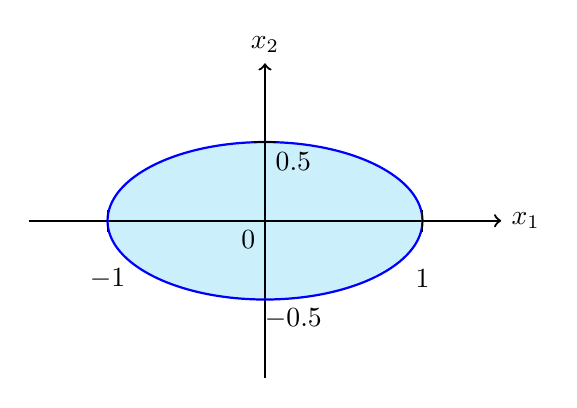
\begin{tikzpicture}[scale=2]
    % Fill the ellipse
    \fill[cyan!20] (0,0) ellipse (1cm and 0.5cm);
    
    % Draw the axes
    \draw[->, thick] (-1.5,0) -- (1.5,0) node[right] {$x_1$};
    \draw[->, thick] (0,-1) -- (0,1) node[above] {$x_2$};
    
    % Draw the ellipse boundary
    \draw[thick, color=blue] (0,0) ellipse (1cm and 0.5cm);
    
    % Add ticks and labels
    \foreach \x in {-1, 1}
        \draw (\x,0.07) -- (\x,-0.07) node[shift={(0, -0.6)}] {$\x$};
    \foreach \y in {-0.5, 0.5}
        \draw (0.07,\y) -- (-0.07,\y) node[shift={(0.5, -0.25)}] {$\y$};
    \node[below left] at (0,0) {$0$};
\end{tikzpicture}
%\caption{The unit ball $\|x\|_w \le 1$ for the weight vector $w=(1,4)$ is an ellipse centered at the origin with semi-major axis of length 1 along the $x_1$-axis and semi-minor axis of length 1/2 along the $x_2$-axis.}
\end{figure}

\subsubsection*{\normalfont}{$\therefore$ The unit ball is an ellipse defined by $x_1^2 + 4x_2^2 \le 1$, with a semi-major axis of length 1 and a semi-minor axis of length 1/2.}

\noindent\rule{\textwidth}{0.4pt}\\

\newpage

%------------------
% Solution for 5
%------------------
\subsection*{Solution 5}
\noindent\rule{\textwidth}{0.4pt}\\
\subsubsection*{Distance Table Discription}
\parbox{\textwidth}{
We are given a set of points $\mathcal{X}=\{A, B, C, D\}$ and a function $d: \mathcal{X} \times \mathcal{X} \to \mathbb{R}$ defined by the following distance table. We will determine if $d$ is a metric by checking the required axioms.
}
\begin{center}
\renewcommand{\arraystretch}{1.2}
\begin{tabular}{c|cccc}
$d(x,y)$ & A & B & C & D \\
\hline
A & 0 & 2 & 1 & 5 \\
B & 2 & 0 & 3 & 4 \\
C & 1 & 3 & 0 & 2 \\
D & 5 & 4 & 2 & 0
\end{tabular}
\end{center}

\subsubsection*{Axiom 1: Non-negativity and Identity of Indiscernibles}
\parbox{\textwidth}{
This axiom requires that $d(x, y) \geq 0$ for all $x, y \in \mathcal{X}$, and that $d(x, y) = 0$ if and only if $x = y$.
\begin{itemize}
    \item \textbf{Non-negativity:} All entries in the table are non-negative, so this condition holds.
    \item \textbf{Identity:} The diagonal entries are all zero, so $d(x, x) = 0$. All off-diagonal entries are strictly positive, so $d(x, y) > 0$ when $x \neq y$.
\end{itemize}
Hence, $d$ satisifies the first axiom (non-negativity \& identity of indiscernibles).
}

\subsubsection*{Axiom 2: Symmetry}
\parbox{\textwidth}{
This axiom requires that $d(x, y) = d(y, x)$ for all $x, y \in \mathcal{X}$. Using the distance table above we can look up the folowiing:
\begin{itemize}
    \item $d(A, B) = 2 = d(B, A)$
    \item $d(A, C) = 1 = d(C, A)$
    \item $d(A, D) = 5 = d(D, A)$
    \item $d(B, C) = 3 = d(C, B)$
    \item $d(B, D) = 4 = d(D, B)$
    \item $d(C, D) = 2 = d(D, C)$
\end{itemize}
Hence, $d$ satisifies the second axiom (symmetry).
}

\subsubsection*{Axiom 3: The Triangle Inequality}
\parbox{\textwidth}{
This axiom requires that for any three points $x, y, z \in \mathcal{X}$, the inequality $d(x, z) \leq d(x, y) + d(y, z)$ must hold. \\
Let $x=A$, $y=C$, and $z=D$.
}
\begin{align*}
    d(x, z) &\leq d(x, y) + d(y, z) \\
    d(A, D) &\leq d(A, C) + d(C, D) \\
    5 &\leq 1 + 2 \\
    5 &\leq 3 \quad (\textbf{False})
\end{align*}
\parbox{\textwidth}{
Hence, the triangle inequality does not hold, and $d$ fails the third axiom.
}

\subsubsection*{\normalfont}{$\therefore$ The function $d$ is not a metric because it fails the triangle inequality.}

\noindent\rule{\textwidth}{0.4pt}\\

\newpage

%------------------
% Solution for 6(a)
%------------------
%%%
\subsection*{Solution 6}
\noindent\rule{\textwidth}{0.4pt}\\
\subsubsection*{Solution 6 (a)}

\subsubsection*{The Largest Possible Value of $K(p, q)$}
\parbox{\textwidth}{
The KL divergence becomes unbounded and approaches infinity if there is an outcome $x \in \mathcal{X}$ that is possible under the true distribution $p$ (i.e., $p(x) > 0$) but is considered impossible by the approximating distribution $q$ (i.e., $q(x) = 0$). This situation violates the condition of absolute continuity. The term $p(x) \log \frac{p(x)}{q(x)}$ becomes infinite, driving the entire sum to infinity. We demonstrate this with two deterministic but opposing distributions.
}
\parbox{\textwidth}{
Let $p=(1, 0)$ and $q=(0, 1)$. This means $p(x_1)=1, p(x_2)=0$ and $q(x_1)=0, q(x_2)=1$.
\begin{align*}
    K(p, q) &= p(x_1) \log\frac{p(x_1)}{q(x_1)} + p(x_2) \log\frac{p(x_2)}{q(x_2)} \\
    &= 1 \cdot \log\frac{1}{0} + 0 \cdot \log\frac{0}{1} \\
    &= \infty + 0 \\
    &= \infty
\end{align*}
}
\subsubsection*{\normalfont}{$\therefore$ The largest possible value of the KL divergence is $\infty$.}


\noindent\rule{\textwidth}{0.4pt}\\

\newpage

%------------------
% Solution for 6(b)
%------------------
%%%
\subsection*{Solution 6}
\noindent\rule{\textwidth}{0.4pt}\\
\subsubsection*{Solution 6 (b)}


\subsubsection*{(b): Proof of Non-Symmetry}
\parbox{\textwidth}{
To prove that the KL divergence is not a symmetric function, we must provide a concrete example where $K(p, q) \neq K(q, p)$. We choose one distribution to be uniform and the other to be deterministic. This highlights the asymmetry in how KL divergence penalizes impossible events.
}
\parbox{\textwidth}{
Let $p = (1/2, 1/2)$ and $q = (1, 0)$. First, we compute $K(p, q)$.
\begin{align*}
    K(p, q) &= p(x_1) \log\frac{p(x_1)}{q(x_1)} + p(x_2) \log\frac{p(x_2)}{q(x_2)} \\
    &= \frac{1}{2} \log\frac{1/2}{1} + \frac{1}{2} \log\frac{1/2}{0} \\
    &= \frac{1}{2} \log\frac{1}{2} + \infty \\
    &= \infty
\end{align*}
Next, we compute the reverse divergence, $K(q, p)$.
\begin{align*}
    K(q, p) &= q(x_1) \log\frac{q(x_1)}{p(x_1)} + q(x_2) \log\frac{q(x_2)}{p(x_2)} \\
    &= 1 \cdot \log\frac{1}{1/2} + 0 \cdot \log\frac{0}{1/2} \\
    &= \log(2) + 0 \\
    &= \log(2)
\end{align*}
}
\subsubsection*{\normalfont}{$\therefore$ Since $K(p, q) = \infty$ and $K(q, p) = \log(2)$, we have shown that $K(p, q) \neq K(q, p)$, and thus KL divergence is not symmetric.}

\noindent\rule{\textwidth}{0.4pt}\\

\newpage

\subsubsection*{\normalfont}{Graduate Level Explanation}
The Kullback-Leibler divergence is a measure of \textbf{relative entropy}, not a distance metric. Its failure to be a metric is fundamental to its interpretation. The non-symmetry shown above is a key property. $K(p, q)$ measures the information lost when $q$ is used to approximate $p$; this is an inherently directional concept.

The unboundedness of $K(p, q)$ is a direct consequence of the violation of \textbf{absolute continuity}. The divergence is finite if and only if the support of $p$ is a subset of the support of $q$ (denoted $\text{supp}(p) \subseteq \text{supp}(q)$ or $p \ll q$). If this condition fails, there exists an event $x$ for which $p(x) > 0$ but $q(x) = 0$. The model $q$ assigns zero probability to an event that can actually occur, leading to an infinite "surprise" or error. This property is crucial in variational inference and Bayesian model comparison, where an infinite divergence signals a catastrophic failure of the approximating distribution to cover the posterior's support. KL divergence is a member of the broader classes of \textit{f-divergences} and \textit{Bregman divergences}, none of which are required to be symmetric. 

\subsubsection*{\normalfont}{Explanation for 5 year old}
Imagine a guessing game. The "Truth" knows the right answer ($p$), and you are making a guess ($q$). The KL divergence is a number that tells us how surprised the Truth is by your guess. A bigger number means more surprise!

\begin{itemize}
    \item \textbf{Why it can be infinite:} The Truth is "The secret animal is a Dog" ($p$ is 100\% Dog). You guess, "I am 100\% certain it's a Cat!" ($q$ is 100\% Cat). You said a Dog was impossible! When the Truth reveals it's a Dog, your surprise is infinite because you were completely wrong about something that was certain.
    
    \item \textbf{Why it's not the same backwards:} Let's look at two cases.
    \begin{enumerate}
        \item The Truth is "The secret animal could be a Dog or a Cat, 50/50 chance" ($p$ is 50/50). You guess, "It's definitely a Dog!" ($q$ is 100\% Dog). The Truth is infinitely surprised because you said a Cat was impossible, but it was possible.
        
        \item Now let's switch! The Truth is "It's definitely a Dog" ($q$ is 100\% Dog). You guess, "It could be a Dog or a Cat, 50/50 chance" ($p$ is 50/50). Is the Truth surprised? A little bit! The Truth is surprised you weren't more confident, but not infinitely surprised, because you at least said a Dog was possible.
    \end{enumerate}
\end{itemize}
Since the surprise is \textbf{infinite} in the first game but just a \textbf{little bit} in the second game, the "surprise-o-meter" doesn't work the same forwards and backwards! 


\newpage

%------------------
% Solution for 7
%------------------
\subsection*{Solution 7}
\noindent\rule{\textwidth}{0.4pt}\\

\subsubsection*{Define Jaccard Similarity}
\parbox{\textwidth}{
Jaccard similarity between two sets $A$ and $B$ is the following:

$$J(A,B) = \frac{|A \cap B|}{|A \cup B|}$$
}
\subsubsection*{Compute Jaccard Similarity}
\parbox{\textwidth}{
Let $A = \{1, 3, 5, 7, 9\}$ and $B = \{2, 3, 5, 7\}$

\begin{align*}
    J(A, B) &= \frac{|A \cap B|}{|A \cup B|} \\
    &= \frac{|\{1, 3, 5, 7, 9\} \cap \{2, 3, 5, 7\}|}{|\{1, 3, 5, 7, 9\} \cup \{2, 3, 5, 7\}|} \\
    &= \frac{|\{3, 5, 7\}|}{|\{1, 2, 3, 5, 7, 9\}|} \\
    &= \frac{3}{6} \\
    &= \frac{1}{2}
\end{align*}
}

\subsubsection*{\normalfont}{$\therefore$ The Jaccard similarity $J(A, B)$ is $\frac{1}{2}$ or 50\%.}

\noindent\rule{\textwidth}{0.4pt}\\

\newpage

\subsection*{Solution 8}
\noindent\rule{\textwidth}{0.4pt}\\
\subsubsection*{Solution: Bigram Jaccard Similarity}
\parbox{\textwidth}{
We are asked to compute the Jaccard similarity based on word bigrams for the following two sentences, where $x'$ is pre-processed to remove punctuation:
\\
$x$: ``Napoleon was born in 1769''
\\
$x'$: ``Napoleon was born when''
\\
The Jaccard similarity for the bigram sets $B(x)$ and $B(x')$ is defined as $J(B(x), B(x')) = \frac{|B(x) \cap B(x')|}{|B(x) \cup B(x')|}$.
}

\subsubsection*{Step 1: Derive Bigram Sets}
\parbox{\textwidth}{
First, we generate the sets of consecutive word pairs (bigrams) for each sentence.
\begin{itemize}
    \item $B(x) = \{(\text{Napoleon, was}), (\text{was, born}), (\text{born, in}), (\text{in, 1769})\}$
    \item $B(x') = \{(\text{Napoleon, was}), (\text{was, born}), (\text{born, when})\}$
\end{itemize}
The sizes of the sets are $|B(x)| = 4$ and $|B(x')| = 3$.
}

\subsubsection*{Step 2: Compute Intersection and Union of Sets}
\parbox{\textwidth}{
Next, we find the intersection (common bigrams) and the union (all unique bigrams) of the two sets.
\begin{itemize}
    \item Intersection: $B(x) \cap B(x') = \{(\text{Napoleon, was}), (\text{was, born})\}$
    \item Union: $B(x) \cup B(x') = \{(\text{Napoleon, was}), (\text{was, born}), (\text{born, in}), (\text{in, 1769}), (\text{born, when})\}$
\end{itemize}
The sizes are $|B(x) \cap B(x')| = 2$ and $|B(x) \cup B(x')| = 5$.
}

\subsubsection*{Step 3: Compute the Jaccard Similarity}
\parbox{\textwidth}{
Finally, we apply the Jaccard similarity formula using the sizes of the intersection and union.
\begin{align*}
    J(B(x), B(x')) &= \frac{|B(x) \cap B(x')|}{|B(x) \cup B(x')|} \\
                  &= \frac{2}{5} \\
                  &= 0.4
\end{align*}
}

\subsubsection*{\normalfont}{$\therefore$ The bigram-based Jaccard similarity between the two sentences is 0.4}

\noindent\rule{\textwidth}{0.4pt}\\

\newpage

\subsubsection*{\normalfont}{Graduate Level Explanation}

\parbox{\textwidth}{
Using Jaccard similarity over n-grams (in this case, bigrams) allows for a measure of text similarity that captures local syntactic and semantic structure, which is a significant improvement over simple bag-of-words models. Unlike methods that treat words as independent, n-grams preserve word order within a small window. This makes the metric sensitive to phrasal correspondence but robust to larger-scale sentence reordering. It is particularly effective for tasks like plagiarism detection, identifying near-duplicate documents, and record linkage, where detecting overlapping text chunks is more important than understanding deep semantic meaning. While it is computationally simpler than embedding-based methods like cosine similarity on BERT vectors, it effectively balances structural awareness with efficiency.
}

\subsubsection*{\normalfont}{Explanation for 5 year old}

\parbox{\textwidth}{
Imagine you and your friend are building sentences with Lego bricks, where each brick is a word.

Instead of just counting how many of the same color bricks you both used, we're going to look at how you connected them. We'll look at every pair of bricks stuck together. A pair of word-bricks is a "bigram".

\begin{enumerate}
    \item First, we find all the two-brick connections that are exactly the same in both of your sentences. Let's say you find \textbf{2} matching connections.
    \item Next, we count all the unique connections you both made. Maybe in total, there are \textbf{5} different connections.
\end{enumerate}

To see how similar your sentences are, we just divide the number of matching connections by the total number of connections: 2 divided by 5. That gives a similarity score! It tells us how much of the sentences were built in the same way.
}

\noindent\rule{\textwidth}{0.4pt}\\

\newpage

\subsection*{Solution 9}
\noindent\rule{\textwidth}{0.4pt}\\
\subsubsection*{Solution 9 (a)}

\subsubsection*{(a): Calculating Cosine Similarity}
\parbox{\textwidth}{
We compute the cosine similarity for the vectors $x = [1, 2, 3]^T$ and $x' = [3, 2, 1]^T$ using the formula $\text{cos}(\theta) = \frac{x \cdot x'}{\|x\|_2 \|x'\|_2}$. First, we compute the dot product and the $\ell_2$-norms.
\\
Dot Product: $x \cdot x' = (1)(3) + (2)(2) + (3)(1)$
\\
Norms: $\|x\|_2 = \sqrt{1^2 + 2^2 + 3^2}$ and $\|x'\|_2 = \sqrt{3^2 + 2^2 + 1^2}$
}
\begin{align*}
    \text{cos}(\theta) &= \frac{(1)(3) + (2)(2) + (3)(1)}{\sqrt{1^2+2^2+3^2} \sqrt{3^2+2^2+1^2}} \\
    &= \frac{3 + 4 + 3}{\sqrt{1+4+9} \sqrt{9+4+1}} \\
    &= \frac{10}{\sqrt{14} \sqrt{14}} \\
    &= \frac{10}{14} \\
    &= \frac{5}{7}
\end{align*}
\subsubsection*{\normalfont}{$\therefore$ The cosine similarity between $x$ and $x'$ is $5/7$.}


\noindent\rule{\textwidth}{0.4pt}\\

\newpage

\subsection*{Solution 9}
\noindent\rule{\textwidth}{0.4pt}\\
\subsubsection*{Solution 9 (b)}
\subsubsection*{(b): Characterization of Zero Similarity}
\parbox{\textwidth}{
The cosine similarity between two non-zero vectors $x$ and $x'$ is zero if and only if the numerator of the formula is zero.
$$ \text{cos}(\theta) = 0 \iff x \cdot x' = 0 $$
In a Euclidean vector space, a dot product of zero signifies that the two vectors are \textbf{orthogonal} (perpendicular) to each other. The angle $\theta$ between them is $90^\circ$ or $\pi/2$ radians. Geometrically, they form a right angle.
}
\subsubsection*{\normalfont}{$\therefore$ A cosine similarity of zero means the vectors are orthogonal.}

\noindent\rule{\textwidth}{0.4pt}\\

\newpage

\subsection*{Solution 9}
\noindent\rule{\textwidth}{0.4pt}\\
\subsubsection*{Solution 9 (c)}


\subsubsection*{(c): Sketch of a High-Similarity Region}
\parbox{\textwidth}{
We want to sketch the region in $\mathbb{R}^2$ where any vector $x'$ has a cosine similarity of at least 0.9 with the vector $x = [1, 2]^T$. The condition is $\text{cos}(\theta) \ge 0.9$, which implies that the angle $\theta$ between $x$ and $x'$ must satisfy $|\theta| \le \arccos(0.9) \approx 25.84^\circ$.
\\~\\
\textbf{Description of the Sketch:}
\begin{itemize}
    \item Draw the standard Cartesian axes, $x_1$ and $x_2$.
    \item Draw the reference vector $x$ as an arrow from the origin $(0,0)$ to the point $(1,2)$.
    \item The region of high similarity is a double-sided cone (a pair of sectors in 2D) centered on the line passing through the origin and the point $(1,2)$.
    \item The cone opens with an angle of $2 \times 25.84^\circ$. Any vector $x'$ that originates at $(0,0)$ and whose tip lies within this cone satisfies the condition.
\end{itemize}
}
\subsubsection*{\normalfont}{$\therefore$ The region is a cone centered on the vector $x$ with an angular radius of $\arccos(0.9)$.}

\noindent\rule{\textwidth}{0.4pt}\\

\newpage

\subsubsection*{\normalfont}{Graduate Level Explanation}

\parbox{\textwidth}{
Cosine similarity is a measure of orientation, not magnitude. By normalizing the vectors to unit length via the $\ell_2$-norm, it isolates the angle between them, making it an effective measure of similarity in applications where vector length is a confounding variable. For instance, in Natural Language Processing, documents are often represented as high-dimensional TF-IDF vectors. A longer document might have a larger Euclidean distance from a shorter one, even if they discuss the same topic. Cosine similarity correctly identifies them as similar by disregarding their "length" (i.e., word count) and focusing solely on their "direction" (i.e., topic, as defined by the distribution of word frequencies). This property is also critical in recommender systems, where it can measure the similarity of user preferences irrespective of the total number of items they have rated.
}

\subsubsection*{\normalfont}{Explanation for 5 year old}

\parbox{\textwidth}{
Imagine you and your friend are each pointing with an arrow. Cosine similarity doesn't care how long your arrows are, only which way they're pointing!
\begin{itemize}
    \item If you both point in the \textbf{exact same direction}, the similarity is \textbf{1}. Perfect match!
    \item If your arrows make a perfect "L" shape (a right angle), the similarity is \textbf{0}. You're not pointing in similar directions at all.
    \item If you point in the \textbf{exact opposite direction} of your friend, the similarity is \textbf{-1}. You completely disagree!
\end{itemize}
It's just a score from -1 to 1 that tells you how much your arrows line up.
}

\newpage

\subsection*{Solution 10}
\noindent\rule{\textwidth}{0.4pt}\\
\subsubsection*{Solution  10 (a)}

\subsubsection*{1 (a): Mean and Median (Theoretical)}
\parbox{\textwidth}{The mean (Expected Value) $E[X]$ is calculated as the sum of each outcome weighted by its probability: $E[X] = \sum_{i} x_i P(X=x_i)$. The median is the value $x_m$ for which the cumulative probability $P(X \le x_m)$ first equals or exceeds 0.5.}
\begin{align*}
E[X] &= (1)\left(\frac{1}{3}\right) + (2)\left(\frac{1}{3}\right) + (3)\left(\frac{1}{12}\right) + (4)\left(\frac{1}{12}\right) + (5)\left(\frac{1}{12}\right) + (6)\left(\frac{1}{12}\right) \\
&= \frac{4}{12} + \frac{8}{12} + \frac{3}{12} + \frac{4}{12} + \frac{5}{12} + \frac{6}{12} \\
&= \frac{30}{12} = \frac{5}{2} = 2.5
\end{align*}
\parbox{\textwidth}{For the median, we find the cumulative probabilities: \\ $P(X \le 1) = 1/3 \approx 0.333$ \\ $P(X \le 2) = 1/3 + 1/3 = 2/3 \approx 0.667$ \\ Since $P(X \le 2)$ is the first cumulative probability to exceed 0.5, the median is 2.}
\subsubsection*{\normalfont}{$\therefore$ The theoretical mean is $E[X] = 2.5$ and the median is $2$.}

\noindent\rule{\textwidth}{0.4pt}\\

\newpage

\subsection*{Solution 10}
\noindent\rule{\textwidth}{0.4pt}\\
\subsubsection*{Solution  10 (b)}

\parbox{\textwidth}{Variance is calculated as $\text{Var}(X) = E[X^2] - (E[X])^2$, where $E[X^2] = \sum_{i} x_i^2 P(X=x_i)$. The standard deviation is the square root of the variance, $\text{SD}(X) = \sqrt{\text{Var}(X)}$.}
\begin{align*}
E[X^2] &= (1^2)\left(\frac{1}{3}\right) + (2^2)\left(\frac{1}{3}\right) + (3^2)\left(\frac{1}{12}\right) + (4^2)\left(\frac{1}{12}\right) + (5^2)\left(\frac{1}{12}\right) + (6^2)\left(\frac{1}{12}\right) \\
&= \frac{4}{12} + \frac{16}{12} + \frac{9}{12} + \frac{16}{12} + \frac{25}{12} + \frac{36}{12} \\
&= \frac{106}{12} = \frac{53}{6} \approx 8.833 \\
\\
\text{Var}(X) &= E[X^2] - (E[X])^2 = \frac{53}{6} - \left(\frac{5}{2}\right)^2 \\
&= \frac{53}{6} - \frac{25}{4} = \frac{106}{12} - \frac{75}{12} = \frac{31}{12} \approx 2.5833 \\
\\
\text{SD}(X) &= \sqrt{\frac{31}{12}} \approx 1.607
\end{align*}
\subsubsection*{\normalfont}{$\therefore$ The theoretical variance is $\text{Var}(X) = 31/12 \approx 2.5833$ and the standard deviation is $\text{SD}(X) \approx 1.607$.}


\noindent\rule{\textwidth}{0.4pt}\\

\newpage

\subsection*{Solution 10}
\noindent\rule{\textwidth}{0.4pt}\\
\subsubsection*{Solution  10 (c)}

\subsubsection*{1 (c): Empirical Probability Distribution}
\parbox{\textwidth}{Given the set of $N=10$ observations $D = \{2, 5, 1, 4, 2, 2, 5, 6, 1, 2\}$, the empirical probability $\hat{P}(X=x)$ for each outcome is its observed frequency divided by the total number of observations, $N$.}
\parbox{\textwidth}{The counts for each outcome are: \\ Count(1) = 2 \\ Count(2) = 4 \\ Count(3) = 0 \\ Count(4) = 1 \\ Count(5) = 2 \\ Count(6) = 1}
\subsubsection*{\normalfont}{$\therefore$ The empirical probabilities are: $\hat{P}(1)=0.2$, $\hat{P}(2)=0.4$, $\hat{P}(3)=0.0$, $\hat{P}(4)=0.1$, $\hat{P}(5)=0.2$, $\hat{P}(6)=0.1$.}


\noindent\rule{\textwidth}{0.4pt}\\

\newpage

\subsection*{Solution 10}
\noindent\rule{\textwidth}{0.4pt}\\
\subsubsection*{Solution  10 (d)}

\subsubsection*{1 (d): Mean, Median, Variance, and SD (Empirical)}
\parbox{\textwidth}{The empirical mean is $\bar{x} = \frac{1}{N}\sum x_i$. The median is the middle value of the sorted data. The empirical variance is $s^2 = \frac{1}{N}\sum(x_i - \bar{x})^2$, and the standard deviation is $s = \sqrt{s^2}$.}
\begin{align*}
\bar{x} &= \frac{1}{10}(2+5+1+4+2+2+5+6+1+2) = \frac{30}{10} = 3.0
\end{align*}
\parbox{\textwidth}{Sorted data: $\{1, 1, 2, 2, \textbf{2, 2}, 4, 5, 5, 6\}$. The median is the average of the 5th and 6th values: $\frac{2+2}{2} = 2$.}
\begin{align*}
s^2 &= \frac{1}{10}\sum_{i=1}^{10}(x_i - 3.0)^2 \\
&= \frac{1}{10}\left[(1-3)^2 \times 2 + (2-3)^2 \times 4 + (4-3)^2 \times 1 + (5-3)^2 \times 2 + (6-3)^2 \times 1\right] \\
&= \frac{1}{10}\left[(-2)^2 \times 2 + (-1)^2 \times 4 + (1)^2 \times 1 + (2)^2 \times 2 + (3)^2 \times 1\right] \\
&= \frac{1}{10}\left[4 \times 2 + 1 \times 4 + 1 \times 1 + 4 \times 2 + 9 \times 1\right] \\
&= \frac{1}{10}\left[8 + 4 + 1 + 8 + 9\right] = \frac{30}{10} = 3.0 \\
\\
s &= \sqrt{3.0} \approx 1.732
\end{align*}
\subsubsection*{\normalfont}{$\therefore$ The empirical mean is $\bar{x}=3.0$, median is $2$, variance is $s^2=3.0$, and standard deviation is $s \approx 1.732$.}


\noindent\rule{\textwidth}{0.4pt}\\

\newpage

\subsubsection*{\normalfont\bf{Graduate Level Explanation: Theoretical vs. Empirical}}
\parbox{\textwidth}{The theoretical distribution describes the true, underlying probability model of the random variable $X$. Its moments, such as the mean $\mu = E[X]$ and variance $\sigma^2 = \text{Var}(X)$, are fixed population parameters derived from this model. The empirical distribution, conversely, is constructed from a finite sample of observations. Its statistics, like the sample mean $\bar{x}$ and sample variance $s^2$, are estimates of the true parameters. The \textbf{Law of Large Numbers (LLN)} states that as the sample size $N$ approaches infinity, the sample mean $\bar{x}$ converges in probability to the theoretical mean $\mu$. Similarly, other empirical moments converge to their theoretical counterparts. The discrepancy between our calculated theoretical values ($\mu=2.5, \sigma^2 \approx 2.58$) and empirical values ($\bar{x}=3.0, s^2=3.0$) is expected due to random sampling variation in our small sample ($N=10$).}


\subsubsection*{\normalfont\bf{Explanation for a 5-Year-Old}}
\parbox{\textwidth}{Imagine you have a magic cookie jar. The \textbf{plan} (the theoretical part) says that for every 12 cookies you pull out, you *should* get 4 chocolate chip, 4 oatmeal, 1 sugar, 1 peanut butter, 1 ginger, and 1 snickerdoodle. The plan's ``average cookie'' is a mix between a chocolate chip and an oatmeal cookie. \\ \\ But then, you actually pull out just 10 cookies. This is your \textbf{handful} (the empirical part). In your handful, you got a lot of oatmeal cookies and no sugar cookies at all! What happened in your one small handful is a little different from the big plan for the whole jar. If you kept pulling out cookies all day (thousands of them!), your handful would start to look a lot more like the original plan.}

\newpage

\subsection*{Solution 11}
\noindent\rule{\textwidth}{0.4pt}\\
\subsubsection*{Solution  11 (a)}

\parbox{\textwidth}{
    \textbf{Justification:} The distribution of human height for a given population (e.g., adult males) is famously well-approximated by a symmetric, bell-shaped curve (a Normal or Gaussian distribution). In a perfectly symmetric distribution, the mean, median, and mode coincide. Therefore, the center of mass (mean) and the geometric center (median) are expected to be nearly identical.
}

\subsubsection*{\normalfont $\therefore$ We expect $\text{Mean}(H) \approx \text{Median}(H)$. No significant difference.}

\noindent\rule{\textwidth}{0.4pt}\\

\newpage

\subsection*{Solution 11}
\noindent\rule{\textwidth}{0.4pt}\\
\subsubsection*{Solution  11 (b)}

\parbox{\textwidth}{
    \textbf{Justification:} The distribution of housing costs is almost always characterized by a strong \textbf{right-skew (positive skew)}. While most houses fall within a certain price range, there is a long tail of extremely expensive properties (mansions, luxury estates). These high-value outliers pull the arithmetic average significantly upward, while the median remains a more robust measure of the "typical" house price, unaffected by these extreme values.
}

\subsubsection*{\normalfont $\therefore$ We expect $\text{Mean}(C) > \text{Median}(C)$. A significant difference.}

\noindent\rule{\textwidth}{0.4pt}\\

\newpage


\subsection*{Solution 11}
\noindent\rule{\textwidth}{0.4pt}\\
\subsubsection*{Solution  11 (c)}

\parbox{\textwidth}{
    \textbf{Justification:} The distribution of GPAs is often \textbf{left-skewed (negative skew)}. This is due to a "ceiling effect," where a large number of students achieve high grades clustered near the maximum possible GPA (e.g., 4.0), while fewer students have very low GPAs. This clustering at the high end pulls the median towards the right, while the lower-end scores pull the mean to the left. However, this skew is often less pronounced than in financial data.
}

\subsubsection*{\normalfont $\therefore$ We expect $\text{Mean}(G) < \text{Median}(G)$, but the difference may not be as significant as for cost or salary.}

\noindent\rule{\textwidth}{0.4pt}\\

\newpage

\subsection*{Solution 11}
\noindent\rule{\textwidth}{0.4pt}\\
\subsubsection*{Solution  11 (d)}

\parbox{\textwidth}{
    \textbf{Justification:} Similar to housing costs, salary data exhibits a pronounced \textbf{right-skew}. The vast majority of people earn salaries within a relatively modest range. However, a small number of individuals (CEOs, top athletes, etc.) have extraordinarily high incomes. These outliers exert a strong influence on the mean, pulling it far to the right of the median. The median salary is therefore a much more accurate representation of a typical worker's earnings.
}
\vspace{1em}
\subsubsection*{\normalfont $\therefore$ We expect $\text{Mean}(S) > \text{Median}(S)$. A significant difference.}


\noindent\rule{\textwidth}{0.4pt}\\

\newpage

\subsubsection*{\normalfont Graduate Level Explanation}
\parbox{\textwidth}{
The \textbf{mean} ($\mu$) is the first moment of a distribution, representing its center of mass. It is defined as the expected value of the random variable $X$, so that $\mu = E[X]$. The mean minimizes the expected squared error, i.e., $\mu = \arg\min_c E[(X-c)^2]$. Its sensitivity to the magnitude of every data point makes it susceptible to being heavily influenced by outliers.

\vspace{0.5em}

The \textbf{median} ($m$) is the value that separates the higher half from the lower half of a data set. More formally, it is a value that minimizes the L1-norm or the expected absolute error, $m = \arg\min_c E[|X-c|]$. This property makes the median a \textbf{robust} estimator of central tendency, as it is insensitive to the magnitude of extreme outliers.

\vspace{0.5em}

In a \textbf{symmetric distribution}, the center of mass and the 50th percentile coincide, thus $\mu = m$. In a \textbf{skewed distribution}, the mass in the tail pulls the mean in its direction. For a right-skewed distribution, the long tail of high-value outliers pulls $\mu > m$. Conversely, for a left-skewed distribution, the tail of low-value outliers pulls $\mu < m$. The median remains a better indicator of the central location of the bulk of the probability mass.
}

\vspace{2em}

\subsubsection*{\normalfont Explanation for a 5-Year-Old}
\parbox{\textwidth}{
Imagine five kids are sharing candy. Four kids get 2 pieces of candy each. But one super-lucky kid gets 50 pieces!

\vspace{0.5em}

If we use the \textbf{mean} (the "average"), we add all the candy up ($2+2+2+2+50 = 58$) and divide by the number of kids (5). The mean is almost 12 pieces per kid! That doesn't sound right, because most kids only got 2. The one kid with 50 pieces pulled the average way up.

\vspace{0.5em}

If we use the \textbf{median} (the "middle"), we line the kids up by how much candy they have: 2, 2, \textbf{2}, 2, 50. The kid in the middle has 2 pieces. The median is 2. This is a much better description of what a typical kid got.

\vspace{0.5em}

So, the \textbf{mean is sensitive} to that one kid with a huge amount of candy (an outlier), while the \textbf{median just looks at the middle} and doesn't care how much the richest kid has.
}

\newpage

\subsection*{Solution 12}
\noindent\rule{\textwidth}{0.4pt}\\
\subsubsection*{nesto ovdje}

\subsubsection*{Question 1: Derivation of the Second Raw Moment}

\parbox{\textwidth}{
The second raw moment, denoted as $E[Z^2]$, can be derived from the first raw moment (the mean, $\mu = E[Z]$) and the second central moment (the variance, $Var[Z] = \sigma^2$) using the fundamental relationship:
$$ Var[Z] = E[Z^2] - (E[Z])^2 $$
Rearranging this formula allows us to solve for $E[Z^2]$:
$$ E[Z^2] = Var[Z] + (E[Z])^2 = \sigma^2 + \mu^2 $$
Given the values $E[Z] = -1$ and the standard deviation $SD[Z] = \sigma = 2$, we can calculate the variance as $\sigma^2 = 2^2 = 4$.
}

\begin{align*}
E[Z^2] &= \sigma^2 + \mu^2 \\
&= (SD[Z])^2 + (E[Z])^2 \\
&= (2)^2 + (-1)^2 \\
&= 4 + 1 \\
&= 5
\end{align*}

\subsubsection*{\normalfont}{$\therefore$ The second raw moment $E[Z^2]$ is 5.}

\noindent\rule{\textwidth}{0.4pt}\\

\subsubsection*{\normalfont}{Graduate Level Explanation}
The relationship $Var(Z) = E[Z^2] - (E[Z])^2$ provides a direct conversion between the second central moment ($Var(Z)$) and the first two raw moments ($E[Z]$ and $E[Z^2]$). In general, central moments, $E[(Z-\mu)^k]$, describe the shape of a distribution relative to its mean, while raw moments, $E[Z^k]$, describe the distribution relative to the origin. This specific formula is a fundamental identity derived from the linearity of expectation and is crucial when working with moment-generating functions (MGFs) or characteristic functions, as raw moments are easily derived from them via differentiation. Physically, in signal processing, if $Z$ represents a random signal, $E[Z]$ is its DC component, and $E[Z^2]$ is related to its total average power. The variance, representing the second central moment, is then interpreted as the AC power of the signal.

\noindent\rule{\textwidth}{0.4pt}\\

\subsubsection*{\normalfont}{Explanation for a 5-Year-Old}
Imagine you are playing a game. Your \textbf{average score} is your mean ($E[Z]$). Let's say your average is -1. How much your scores jump around from that average is the \textbf{wildness} (standard deviation, $\sigma$). Let's say the wildness is 2. We want to find the "average of the scores squared" ($E[Z^2]$). To get this, you just follow a simple rule: combine the \textbf{wildness squared} with the \textbf{average score squared}.
$$ \text{Average Score Squared} = (\text{Wildness})^2 + (\text{Average Score})^2 $$
So, we calculate $(2 \times 2) + (-1 \times -1) = 4 + 1 = 5$. It's a fundamental statistical rule that connects how spread out your scores are with what your average score is.



\noindent\rule{\textwidth}{0.4pt}\\

\newpage

\subsection*{Solution 13}
\noindent\rule{\textwidth}{0.4pt}\\
\subsubsection*{Solution  13 (a)}

\subsubsection*{Part (a): Are X and Y Independent?}

\parbox{\textwidth}{
Two discrete random variables $X$ and $Y$ are independent if and only if $P(X=x, Y=y) = P(X=x)P(Y=y)$ for all possible pairs $(x, y)$. A single counterexample is sufficient to prove dependence. First, we compute the marginal probability mass functions, $P(X=x)$ and $P(Y=y)$, by summing the rows and columns of the joint PMF table, respectively.
\begin{align*}
    P(X=1) &= 0.10 + 0.20 + 0.05 = 0.35 \\
    P(X=2) &= 0.10 + 0.15 + 0.05 = 0.30 \\
    P(X=3) &= 0.10 + 0.15 + 0.10 = 0.35
\end{align*}
\begin{align*}
    P(Y=1) &= 0.10 + 0.10 + 0.10 = 0.30 \\
    P(Y=2) &= 0.20 + 0.15 + 0.15 = 0.50 \\
    P(Y=3) &= 0.05 + 0.05 + 0.10 = 0.20
\end{align*}
}
\vspace{1em}

We test the independence condition for the pair $(X=1, Y=1)$:
\begin{align*}
    P(X=1, Y=1) &\stackrel{?}{=} P(X=1)P(Y=1) \\
    0.10 &\stackrel{?}{=} (0.35)(0.30) \\
    0.10 &\neq 0.105
\end{align*}

\subsubsection*{\normalfont{$\therefore$ Since the joint probability $P(X=1, Y=1)$ does not equal the product of the marginal probabilities $P(X=1)P(Y=1)$, the random variables $X$ and $Y$ are NOT independent.}}

\noindent\rule{\textwidth}{0.4pt}\\

\newpage

\subsection*{Solution 13}
\noindent\rule{\textwidth}{0.4pt}\\
\subsubsection*{Solution  13 (b)}

\subsubsection*{Part (b): What are the Covariance and Correlation of X and Y?}

\parbox{\textwidth}{
To find the covariance and correlation, we must first compute the expectations $E[X]$, $E[Y]$, and $E[XY]$. The covariance is then given by $\text{Cov}[X, Y] = E[XY] - E[X]E[Y]$, and the correlation is $\rho_{X, Y} = \frac{\text{Cov}[X, Y]}{\sigma_X \sigma_Y}$.
}
\vspace{1em}

\textbf{1. Calculate Expectations:}
\begin{align*}
    E[X] &= \sum_{x} x P(X=x) \\
         &= 1(0.35) + 2(0.30) + 3(0.35) \\
         &= 0.35 + 0.60 + 1.05 = \mathbf{2.0} \\
    \\
    E[Y] &= \sum_{y} y P(Y=y) \\
         &= 1(0.30) + 2(0.50) + 3(0.20) \\
         &= 0.30 + 1.00 + 0.60 = \mathbf{1.9} \\
    \\
    E[XY] &= \sum_{x,y} xy P(X=x, Y=y) \\
          &= (1)(1)(0.10) + (1)(2)(0.20) + (1)(3)(0.05) \\
          &\quad + (2)(1)(0.10) + (2)(2)(0.15) + (2)(3)(0.05) \\
          &\quad + (3)(1)(0.10) + (3)(2)(0.15) + (3)(3)(0.10) \\
          &= 0.10 + 0.40 + 0.15 + 0.20 + 0.60 + 0.30 + 0.30 + 0.90 + 0.90 \\
          &= \mathbf{3.85}
\end{align*}

\textbf{2. Calculate Covariance:}
\begin{align*}
    \text{Cov}[X, Y] &= E[XY] - E[X]E[Y] \\
                   &= 3.85 - (2.0)(1.9) \\
                   &= 3.85 - 3.80 = \mathbf{0.05}
\end{align*}

\textbf{3. Calculate Variances and Standard Deviations:}
\begin{align*}
    E[X^2] &= 1^2(0.35) + 2^2(0.30) + 3^2(0.35) = 0.35 + 1.20 + 3.15 = 4.7 \\
    \text{Var}[X] &= E[X^2] - (E[X])^2 = 4.7 - 2.0^2 = 0.7 \\
    \sigma_X &= \sqrt{0.7} \approx 0.8367 \\
    \\
    E[Y^2] &= 1^2(0.30) + 2^2(0.50) + 3^2(0.20) = 0.30 + 2.00 + 1.80 = 4.1 \\
    \text{Var}[Y] &= E[Y^2] - (E[Y])^2 = 4.1 - 1.9^2 = 4.1 - 3.61 = 0.49 \\
    \sigma_Y &= \sqrt{0.49} = 0.7
\end{align*}

\textbf{4. Calculate Correlation Coefficient:}
\begin{align*}
    \rho_{X, Y} &= \frac{\text{Cov}[X, Y]}{\sigma_X \sigma_Y} \\
               &= \frac{0.05}{\sqrt{0.7} \cdot \sqrt{0.49}} \\
               &= \frac{0.05}{(0.8367)(0.7)} \\
               &\approx \frac{0.05}{0.5857} \approx \mathbf{0.0854}
\end{align*}

\subsubsection*{\normalfont{$\therefore$ The covariance is $\text{Cov}[X, Y] = 0.05$, and the correlation coefficient is $\rho_{X, Y} \approx 0.0854$. This indicates a very weak positive linear relationship between $X$ and $Y$.}}

\noindent\rule{\textwidth}{0.4pt}\\

\newpage

\subsubsection*{\normalfont{Graduate Level Explanation}}
Two random variables $X$ and $Y$ are independent if and only if the $\sigma$-algebras they generate, $\sigma(X)$ and $\sigma(Y)$, are independent. For discrete variables, this is equivalent to the factorization of the joint PMF, $p_{X,Y}(x,y) = p_X(x)p_Y(y)$, for all $(x,y)$ in the support.
\\ \\
Covariance and correlation are measures of the \textbf{linear dependence} between two random variables. A non-zero correlation implies dependence, but the converse is not true. Two variables can be functionally dependent yet have zero correlation if the relationship is non-linear. For example, if $X \sim \text{Uniform}\{-1, 0, 1\}$ and $Y=X^2$, then $X$ and $Y$ are clearly dependent. However, $E[X]=0$ and $E[XY]=E[X^3]=0$, so $\text{Cov}[X,Y]=0$. In this problem, because $\text{Cov}[X,Y] \neq 0$, we have a second confirmation that $X$ and $Y$ are dependent. The joint PMF is the most fundamental description, as it fully defines the probability measure for the random vector $(X, Y)$ and allows for the computation of any property, including marginals, conditionals, and moments.

\noindent\rule{\textwidth}{0.4pt}\\

\subsubsection*{\normalfont{Explanation for a 5-Year-Old}}
Imagine two friends, Alex (who is variable X) and Ben (who is variable Y). They each have a bag with balls numbered 1, 2, and 3.
\\ \\
\textbf{Independence}: If they are ``independent,'' it means that when Alex picks a number, it tells you \textit{nothing} about what number Ben is likely to pick. Knowing Alex picked a `3` doesn't make it any more or less likely that Ben will pick a `1`, `2`, or `3`. In our problem, we found out they are \textbf{not} independent. This means that knowing what number Alex picks gives you a small hint about what Ben might pick.
\\ \\
\textbf{Correlation}: This is a number that tells us \textit{how much} Alex's choice is connected to Ben's choice.
\begin{itemize}
    \item If the number is close to \textbf{+1}, it means they are best buddies. When Alex picks a high number (like 3), Ben is very likely to pick a high number too.
    \item If the number is close to \textbf{-1}, they are opposites. When Alex picks a high number, Ben is very likely to pick a low number (like 1).
    \item If the number is close to \textbf{0}, it means there isn't a clear "high-high" or "high-low" pattern.
\end{itemize}
We found a number that is very, very close to 0 (it was 0.0854). This means that while Alex and Ben are not totally independent, there is only a tiny, tiny hint of a pattern where if one picks a higher number, the other one might also pick a slightly higher number. But the connection is so weak, it's almost not there.


\newpage

\subsection*{Solution 14}
\noindent\rule{\textwidth}{0.4pt}\\
\subsubsection*{Solution  14 (a)}
\subsubsection*{Part (a): Deriving the Covariance $\text{Cov}[X, Y]$}
\parbox{\textwidth}{
We begin by finding the expectation of $Y$, $E[Y]$, using the linearity of expectation:
$$ E[Y] = E[aX + b] = aE[X] + b $$
The covariance between $X$ and $Y$ is defined as $\text{Cov}[X, Y] = E[(X - E[X])(Y - E[Y])]$. Substituting the expression for $E[Y]$, we derive the covariance as follows:
}
\begin{align*}
\text{Cov}[X, Y] &= E\left[ (X - E[X])(Y - E[Y]) \right] \\
&= E\left[ (X - E[X])((aX + b) - (aE[X] + b)) \right] \\
&= E\left[ (X - E[X])(aX + b - aE[X] - b) \right] \\
&= E\left[ (X - E[X])(aX - aE[X]) \right] \\
&= E\left[ (X - E[X])a(X - E[X]) \right] \\
&= a \cdot E\left[ (X - E[X])^2 \right] \\
&= a \cdot \text{Var}[X]
\end{align*}

\subsubsection*{\normalfont}{$\therefore$ The covariance between $X$ and $Y$ is $\text{Cov}[X, Y] = a \cdot \text{Var}[X]$.}


\noindent\rule{\textwidth}{0.4pt}\\

\newpage

\subsection*{Solution 14}
\noindent\rule{\textwidth}{0.4pt}\\
\subsubsection*{Solution  14 (b)}

\subsubsection*{Part (b): Deriving the Correlation $\rho_{X, Y}$}
\parbox{\textwidth}{
The correlation coefficient $\rho_{X, Y}$ is defined as $\rho_{X, Y} = \frac{\text{Cov}[X, Y]}{\text{SD}[X]\text{SD}[Y]}$. We first need to find the standard deviation of $Y$, $\text{SD}[Y]$.
$$ \text{Var}[Y] = \text{Var}[aX + b] = a^2 \text{Var}[X] $$
$$ \text{SD}[Y] = \sqrt{\text{Var}[Y]} = \sqrt{a^2 \text{Var}[X]} = |a|\sqrt{\text{Var}[X]} = |a| \cdot \text{SD}[X] $$
Now we substitute the known quantities into the correlation formula:
}
\begin{align*}
\rho_{X, Y} &= \frac{\text{Cov}[X, Y]}{\text{SD}[X]\text{SD}[Y]} \\
&= \frac{a \cdot \text{Var}[X]}{\text{SD}[X] \cdot (|a| \cdot \text{SD}[X])} \\
&= \frac{a \cdot (\text{SD}[X])^2}{|a| \cdot (\text{SD}[X])^2} \\
&= \frac{a}{|a|} \\
&= \text{sgn}(a)
\end{align*}

\subsubsection*{\normalfont}{$\therefore$ The correlation between $X$ and $Y$ is $\rho_{X, Y} = \text{sgn}(a)$, which is $1$ if $a>0$, $-1$ if $a<0$, and undefined if $a=0$.}


\noindent\rule{\textwidth}{0.4pt}\\

\newpage

\subsubsection*{\normalfont}{Graduate Level Explanation}
The result $\rho_{X, Y} = \pm 1$ provides a foundational insight into the nature of the Pearson correlation coefficient. Correlation measures the strength and direction of a \textbf{linear relationship} between two variables. Since $Y=aX+b$ is, by definition, a perfect linear function of $X$, the magnitude of the correlation must be maximal, which is 1. The sign of the correlation is determined entirely by the slope of the line, $a$. A positive slope ($a>0$) means $X$ and $Y$ move in the same direction, yielding $\rho_{X,Y}=1$. A negative slope ($a<0$) means they move in opposite directions, yielding $\rho_{X,Y}=-1$.

It is critical to note that the additive constant, $b$, has no impact on the final correlation. This is because correlation, like covariance and variance, is a measure of spread and co-movement, not of location. The term $b$ simply shifts the mean of $Y$ ($E[Y] = aE[X] + b$) but does not alter its variance ($\text{Var}[Y] = a^2\text{Var}[X]$). Since the correlation coefficient is standardized by the variables' standard deviations, it is invariant to shifts in location.

\subsubsection*{\normalfont}{Explanation for a 5-Year-Old}
Imagine you have a magic growing toy ($X$). Every year it gets older, it also gets taller in a very specific way. Let's say for every 1 year it gets older ($X$), it grows exactly 3 inches taller ($Y$). So, $Y = 3X$.

If you know the toy's age, you know its height perfectly! They are perfectly linked together. When its age goes up, its height \textbf{must} go up. This perfect link is what we call a correlation of \textbf{1}. It's the highest score you can get!

Now, what if we started measuring the toy from a small stool that is 10 inches tall? The rule becomes $Y = 3X + 10$. The toy is always 10 inches taller than before, but the way it grows each year doesn't change. It still grows exactly 3 inches for every 1 year. The link between its age and growth is still perfect. The $+10$ is like the stool ($b$)—it changes the starting point but not the relationship.

If the magic toy got shorter as it got older (a weird toy!), the link would still be perfect, but it would be going in the opposite direction. That would be a perfect negative link, which is a correlation of \textbf{-1}.


\newpage

\subsection*{Solution 15}
\noindent\rule{\textwidth}{0.4pt}\\
\subsubsection*{nesto ovdje}

\parbox{\textwidth}{
    Let $X$ be a discrete random variable with the sample space $\Omega_X = \{-1, 0, 1\}$ and a uniform probability mass function $P(X=x) = \frac{1}{3}$ for all $x \in \Omega_X$. Find a non-trivial function $Y = f(X)$ such that $X$ and $Y$ are deterministically dependent but have zero covariance, i.e., $\text{Cov}[X, Y] = 0$.
}

\vspace{1em}
\noindent\rule{\textwidth}{0.4pt}\\

\subsubsection*{Part 1: Determine E[X] and Simplify the Covariance Condition}
\parbox{\textwidth}{
    Two random variables $X$ and $Y$ are uncorrelated if their covariance is zero. The covariance is defined as:
    $$ \text{Cov}[X, Y] = E[XY] - E[X]E[Y] $$
    We first calculate the expected value of $X$, $E[X]$.
}
\begin{align*}
    E[X] &= \sum_{x \in \Omega_X} x \cdot P(X=x) \\
         &= (-1) \cdot P(X=-1) + (0) \cdot P(X=0) + (1) \cdot P(X=1) \\
         &= (-1) \cdot \frac{1}{3} + (0) \cdot \frac{1}{3} + (1) \cdot \frac{1}{3} \\
         &= -\frac{1}{3} + 0 + \frac{1}{3} \\
         &= 0
\end{align*}
\parbox{\textwidth}{
    Since $E[X] = 0$, the covariance formula simplifies significantly:
    $$ \text{Cov}[X, Y] = E[XY] - (0) \cdot E[Y] = E[XY] $$
    Therefore, for $X$ and $Y$ to be uncorrelated, we only need to find a function $f$ such that $\mathbf{E[X f(X)] = 0}$.
}

\vspace{1em}
\noindent\rule{\textwidth}{0.4pt}\\

\subsubsection*{Part 2: Derive and Test the Function $f(X)$}
\parbox{\textwidth}{
    The condition $E[X f(X)] = 0$ expands to:
    $$ E[X f(X)] = \sum_{x \in \Omega_X} x f(x) P(X=x) = \frac{1}{3} \left( (-1)f(-1) + (0)f(0) + (1)f(1) \right) = 0 $$
    This implies that we need $-f(-1) + f(1) = 0$, or $\mathbf{f(-1) = f(1)}$. A simple, non-linear function that satisfies this condition is the quadratic function $f(x) = x^2$. Let's define $Y = X^2$ and verify that $E[XY] = 0$.
}
\begin{align*}
    E[XY] &= E[X \cdot X^2] = E[X^3] \\
          &= \sum_{x \in \Omega_X} x^3 \cdot P(X=x) \\
          &= (-1)^3 \cdot P(X=-1) + (0)^3 \cdot P(X=0) + (1)^3 \cdot P(X=1) \\
          &= (-1) \cdot \frac{1}{3} + (0) \cdot \frac{1}{3} + (1) \cdot \frac{1}{3} \\
          &= -\frac{1}{3} + 0 + \frac{1}{3} \\
          &= 0
\end{align*}
\parbox{\textwidth}{
    Since $E[XY] = 0$ and $E[X]=0$, we have $\text{Cov}[X, Y] = 0$. The variable $Y=X^2$ is perfectly determined by $X$, yet they are linearly uncorrelated.
}

\vspace{1em}
\noindent\rule{\textwidth}{0.4pt}\\

\subsubsection*{\normalfont{$\therefore$ Final Answer}}
A suitable function is $\mathbf{Y = f(X) = X^2}$.

\vspace{1em}
\noindent\rule{\textwidth}{0.4pt}\\

\subsubsection*{\normalfont{Graduate Level Explanation}}
\parbox{\textwidth}{
    Covariance and its normalized counterpart, the Pearson correlation coefficient ($\rho_{X,Y}$), are measures of \textbf{linear dependence} only. They quantify the strength and direction of a linear relationship between two variables. In this case, the relationship $Y=X^2$ is perfectly deterministic but also perfectly non-linear (it is parabolic). The distribution of $X$ is symmetric about the origin, which means its first moment, $E[X]$, is zero. The covariance calculation hinges on the third moment, $E[X^3]$, because $E[XY] = E[X \cdot X^2] = E[X^3]$. Due to the symmetry of the underlying distribution of $X$, the negative contribution from $X=-1$ (i.e., $(-1)^3 = -1$) exactly cancels the positive contribution from $X=1$ (i.e., $1^3 = 1$). This results in $E[X^3]=0$ and thus $\text{Cov}[X,Y]=0$. This is a canonical example of \textbf{uncorrelated dependence}, illustrating that a lack of linear correlation does not imply statistical independence. Independence implies zero covariance, but the converse is not true.
}

\vspace{1em}
\noindent\rule{\textwidth}{0.4pt}\\

\subsubsection*{\normalfont{Explanation for a 5-Year-Old}}
\parbox{\textwidth}{
    Imagine two friends, Xavier (X) and Yasmin (Y). They have a secret rule: Yasmin's number is always Xavier's number multiplied by itself ($Y = X \times X$). So if Xavier picks -1, Yasmin's number must be 1. If Xavier picks 1, Yasmin's number must also be 1. Yasmin's number is perfectly predictable from Xavier's.
    \newline\newline
    Now, "correlation" is a way to ask: when Xavier's number goes up, does Yasmin's number also tend to go up? Or does it go down? We are only checking if they follow a straight line together.
    \newline\newline
    But look at their game. When Xavier goes from -1 to 0, his number goes up, but Yasmin's number goes down (from 1 to 0). But when Xavier goes from 0 to 1, his number goes up, and Yasmin's number also goes up (from 0 to 1). They don't stick to a simple "go up together" or "one goes up, one goes down" rule. Because their relationship isn't a straight line, the correlation calculator gets confused and says "zero correlation!" even though they are perfectly linked by their secret rule.
}

\noindent\rule{\textwidth}{0.4pt}\\

\end{document}